
\section{Samples and Simulation}\label{sec:sims}

\begin{figure}
    \centering
    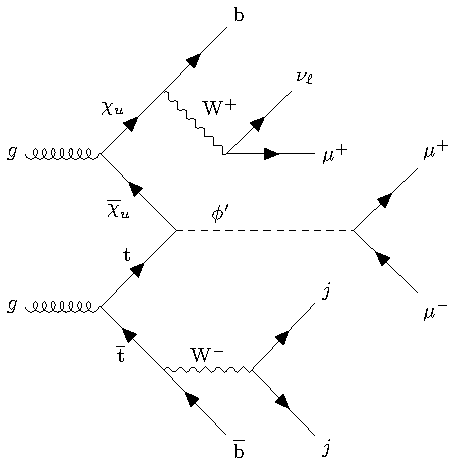
\includegraphics[width=0.75\linewidth]{Images/signal_qqfusion.pdf}
    \caption{Representative Feynman diagram for the production of a $\phi'$ boson in association with a $\chi_\mathrm{u}$ vector-like quark through the fusion of a top quark and $\chi_\mathrm{u}$ vector-like quark. Once again, the $\phi'$ decays to a pair of muons, the top quark decays fully hadronically, and the $\chi_\mathrm{u}$ decays semi-leptonically to muons, neutrinos and $b$-jets.\label{fig:qqfusion}}
\end{figure}

\begin{figure}
    \centering
    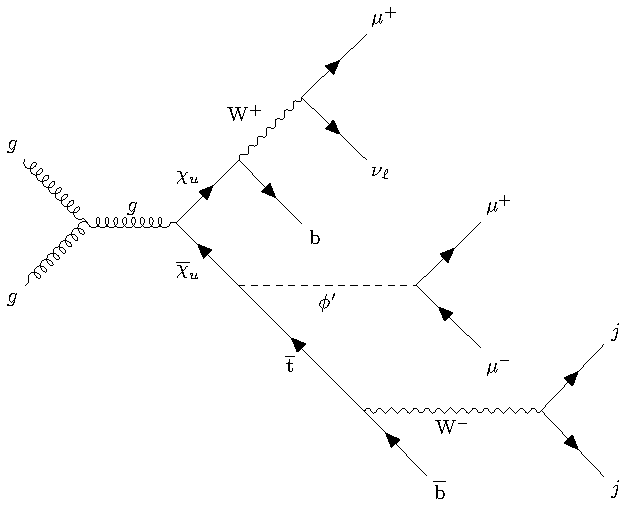
\includegraphics[width=0.85\linewidth]{Images/signal_ggfusion.pdf}
    \caption{Representative Feynman diagram for the production of a $\phi'$ boson in association with a $\chi_\mathrm{u}$ vector-like quark through the fusion of a gluon pair from incoming protons. The $\phi'$ decays to a pair of muons, the top quark that decays fully hadronically, and the $\chi_\mathrm{u}$ decay semi-leptonically to muons, neutrinos and jets.\label{fig:ggfusion}}
\end{figure}

The minimal $U(1)_{T^3_R}$ model described in Sec.~\ref{sec:model} is implemented \textit{at tree level} into the \texttt{FeynRules} package~\parencite{Alloul:2013bka}, which generates the Feynman rules and exports them into a Universal \texttt{FeynRules} Output (\texttt{UFO})~\parencite{Degrande:2011ua}. The resulting \texttt{UFO} is utilized as input for a generator to produce the MC samples. Both signal and background events are generated with the \texttt{MadGraph5\_aMC@NLO} v3.2.0 program~\parencite{Alwall:2014hca,Alwall:2014bza} at leading order (LO) in QCD, considering \textrm{pp} beams colliding with a center-of-mass energy of $\sqrt{s} = 13.6$ \textrm{TeV}. Each signal and background sample is generated separately, with no interference effects between the signal and background considered. The impact of these interference effects has been evaluated, and for all values of $\chi_\mathrm{u}$ and $\phi'$ masses considered, the effect on the signal plus background cross section is found to be less than $<0.5$\%. Additionally, the effect on the shape of the b-jet $p_{T}$ distribution is less than 6\% for $p_{T} < 300$ GeV and less than 2\% for b-jet $p_{T} > 300$ GeV. We use the \texttt{NNPDF3.0~NLO}~\parencite{NNPDF:2014otw} set for parton distribution functions (PDFs) for all event generation. Parton-level events are then interfaced with \texttt{PYTHIA} (v8.2.44)~\parencite{Sjostrand:2014zea} to account for parton showering and hadronization processes. Finally, we use  \texttt{DELPHES} (v3.4.2)~\parencite{deFavereau:2013fsa} to simulate smearing and other detector effects using the CMS detector geometric configurations and parameters for particle identification and reconstruction, using the CMS input card with 140 average pileup interactions. All signal cross sections used in this analysis are obtained requiring the following kinematic criteria on leptons $\ell$, \textrm{b} quarks, and light-quark/gluon jets ($j$) at parton level in \texttt{MadGraph}: $p_{\mathrm{T}}(\ell) > 35$~\textrm{GeV}, $\abs{\eta (\mathrm{b})} < 2.5$, $\abs{\eta (\ell)} < 2.3$, $p_{\mathrm{T}}(j) > 20$~\textrm{GeV}, and $\abs{\eta (\mathrm{j})} < 5$. These parton-level selections were applied exclusively to the signal processes to restrict event generation to the relevant phase space regions. For background processes, these default parton level requirements in \texttt{MadGraph} were imposed:  $p_{\mathrm{T}}(\ell) > 10$~\textrm{GeV}, $\abs{\eta (\ell)} < 2.5$, $p_{\mathrm{T}}(j) > 20$~\textrm{GeV}, $\abs{\eta (\mathrm{j})} < 5$, and $\abs{\eta (\mathrm{b})} < 5$. This ensures that the phase space regions for the background near the analysis-level selection criteria are adequately described after parton showering since the pre-selections at the analysis level are more stringent than the parton-level requirements. Furthermore, we use the MLM algorithm for jet matching and jet merging. The parameters \texttt{xqcut} and \texttt{qcut} of the MLM algorithm are set to 30 and 45 respectively to ensure continuity of the differential jet rate as a function of jet multiplicity. Each simulated signal and background sample is produced separately at LO, with one million events at the generation level, neglecting potential interference effects between the signal and background due to the suppression caused by the different orders of magnitude in the coupling constants of the signal and background.

Signal samples are generated considering the production of a $\phi'$ boson, an associated $\chi_\mathrm{u}$ vector-like quark, and a top quark $(\mathrm{pp}\to \chi_\mathrm{u} \mathrm{t} \phi')$, inclusive in both $\alpha$ and $\alpha_s$ (see Figures~\ref{fig:qqfusion}-\ref{fig:ggfusion}). We have used the implementation of the $U(1)_{T^3_R}$ model in Ref.~\parencite{Dutta2023}. Signal samples were created considering coupling values of $Y_{\mathrm{t}_R}=Y_{\mathrm{t}_L}=2\sqrt{2}$ in the range of masses $m(\phi')\in\{5,10,50,100,325\}$~\textrm{GeV} for the dark higgs and $m(\chi_\mathrm{u})\in\{0.50, 0.75, 1.0, 1.5, 2.0, $ $ 2.5\}$~\textrm{TeV} for the vector-like quark $\chi_u$~\parencite{PhysRevD.108.095006}. The production cross section for $\mathrm{pp}\to \chi_\mathrm{u} \mathrm{t} \phi'$ is highly dependent on the choice of the Yukawa couplings in the Lagrangian. The ${\chi_\mathrm{u}}{- \mathrm{t}}$ fusion process shown in Figure~\ref{fig:qqfusion} is dominated by the $Y_{\mathrm{t}_R}$ coupling. However, the decay ${\chi_\mathrm{u}} \to \mathrm{t} \phi'$ shown in Figure~\ref{fig:ggfusion} is inversely proportional to the $Y_{\mathrm{t}_L}$ coupling. This effect is shown in Figure~\ref{fig:cross_section_by_lambdas}, which displays the total signal cross section, as a function of $Y_{\mathrm{t}_R}$ and $Y_{\mathrm{t}_L}$, for a benchmark point with $m(\phi')=100$~\textrm{GeV} and $m(\chi_\mathrm{u})=1.0$~\textrm{TeV}. 

\begin{figure}
    \centering
    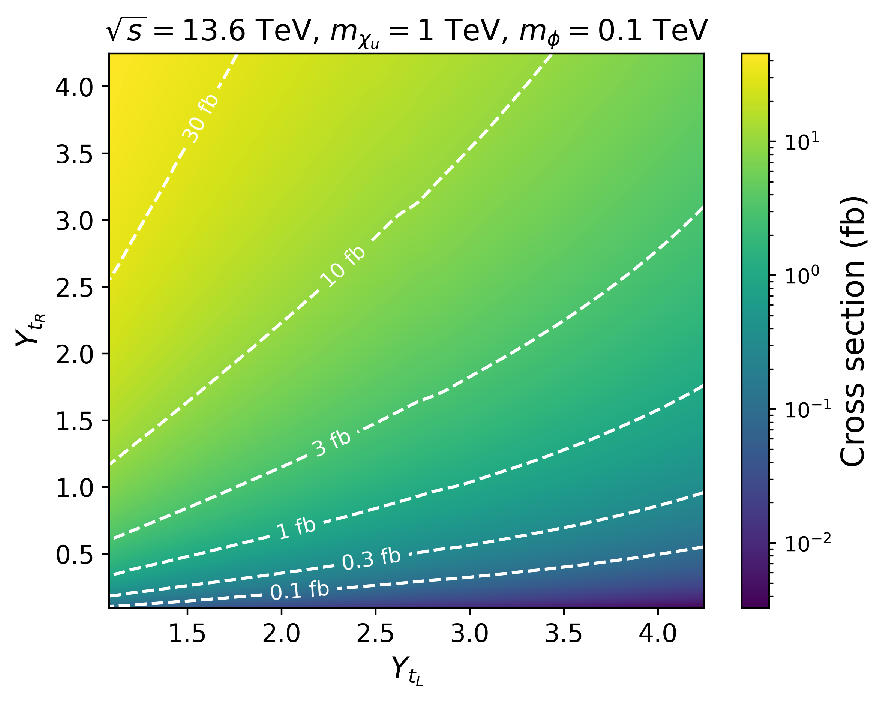
\includegraphics[width=0.85\linewidth]{Images/cross_section_by_lambdas.pdf}
    \caption{Signal production cross section, $ \mathrm{pp}\to \chi_\mathrm{u} \mathrm{t} \phi'$,  in the $Y_{\mathrm{t}_R}$ versus $Y_{\mathrm{t}_L}$ plane, for a benchmark point with $m(\phi')=100$~\textrm{GeV} and $m(\chi_\mathrm{u})=1.00$~\textrm{TeV}. The white-dashed contours show specific cross section values in the two dimensional plane.}
    \label{fig:cross_section_by_lambdas}
\end{figure}

We target signal events where the top quark decays hadronically into a bottom quark and two jets ($\mathrm{t} \to \mathrm{bW} \to \mathrm{b} q \bar{q}'$), the $\chi_\mathrm{u}$ decays semileptonically into a $b$ quark, lepton, and neutrino (via $\chi_\mathrm{u} \to \mathrm{bW}$ and $\mathrm{W}\to\mu\nu_{\mu}$), and the $\phi'$ produces two muons. We note that the scalar $\phi'$ particle could result from the mixture of the SM Higgs boson and additional scalar fields, and the Yukawas of the fermions could additionally arise from the mixing of the SM fermions with additional copies of the associated vector-like fermions. Therefore, the $\phi'$ branching ratios are dependent on the chosen mechanism and model by which this mixture occurs, see for example, Refs.~\parencite{Cacciapaglia_2023,Blankenburg:2012nx,Jones-Perez:2013oia,Calibbi:2009pv}. For the purpose of this work, and 
similar to Refs.~\parencite{Dutta2020,Dutta2023}, the considered benchmark signal scenarios have $\mathfrak{B}(\chi_\mathrm{u} \rightarrow \textrm{b W})$ of about 0.5 and $\mathfrak{B}(\phi' \rightarrow \mu^+\mu^-)=1.00$. Figure~\ref{fig:xs-plot} shows the production cross section in \textrm{fb}, as a function of $m(\phi')$ and $m(\chi_\mathrm{u})$ masses, assuming the aforementioned decays, branching ratios, and couplings.

We note that for the parameter space of focus in this paper, the total mass of the $t$-$\chi_\mathrm{u}$ system is larger than $m(\phi')$, thus the large rest energy of the $t$-$\chi_\mathrm{u}$ system is converted into potentially large momentum values for the $\phi'$. Similarly, the $t$-quark produced through the $\chi_\mathrm{u}$-$t$ fusion interaction can also have large momentum values, and thus in some cases the hadronic $t$ decay products cannot be fully reconstructed independently of each other. This results in three possible $t$ reconstruction scenarios: a fully merged scenario where the $\mathrm{W}\to jj$ system and the $\mathrm{b}$ quarks are very collimated and reconstructed as a single ``fat jet’’ (henceforth referred to as a FatJet, FJ); a partially merged scenario, where the decay products of the $\mathrm{W}$ boson form a single FatJet but the $\mathrm{b}$ quark can still be separately identified; and an un-merged scenario where all decay products can be independently identified. Jets are clustered using the anti-$k_t$ algorithm~\parencite{Cacciari_2008} using the \texttt{FastJet} (v3.4.2)~\parencite{Cacciari_2012} package with a distance parameter of $R = 0.4$ for standard jets and $R = 0.8$ for fat jet objects. Each scenario has an associated identification efficiency and misidentification rate, which depends on the choice of the boosted $t$/$W$ algorithm (our choice of efficiency and misidentification rates is described later). 

Based on the above details, the final state of interest in this paper consists of three muons (two from the $\phi'$ decay and one from the $\chi_\mathrm{u}$ decay), a (possibly boosted) top-tagged system, at least one $b$-tagged jet, and large missing transverse momentum ($\vec{p}_{T}^{\textrm{~miss}}$). For the partially merged and un-merged scenarios, there will be two $b$ quarks present in the final state (one of which is part of the top tagged system). 

We consider background sources from SM processes which can give similar objects in the final state as those expected for signal. Several background sources were considered and studied, such as QCD multijet events, production of vector boson pairs ($\mathrm{VV: WW, ZZ, WZ}$), vector boson triplets ($\mathrm{VVV: WWZ, WZZ, ZZZ, WWW}$), top-quark pairs in association with weak bosons ($\mathrm{t}\overline{\mathrm{t}}X$), and $\mathrm{t}\overline{\mathrm{t}}\mathrm{t}\overline{\mathrm{t}}$ processes. The  dominant sources of SM background events are from the $\mathrm{t}\overline{\mathrm{t}}X$, $\mathrm{ZZW}$, and $\mathrm{t}\overline{\mathrm{t}}\mathrm{t}\overline{\mathrm{t}}$ processes. The $\mathrm{t}\overline{\mathrm{t}}X$ background is primarily associated production of a $\mathrm{Z}/\gamma^{*}$ from $\mathrm{t}\bar{\mathrm{t}}$ fusion processes. The $\mathrm{ZZW}$ process becomes a background when one $\mathrm{Z}$ decays $\mathrm{b}\bar{\mathrm{b}}$, another $\mathrm{Z}$ decays to a pair of muons, and the W decays to a muon and a neutrino. 
Events from $\mathrm{ZZW}$ and $\mathrm{t}\overline{\mathrm{t}}\mathrm{t}\overline{\mathrm{t}}$ have been combined, after being weighted by their corresponding production cross section. The combination is presented as the ``$\mathrm{b} \overline{\mathrm{b}}\mu\mu\mu\nu$'' background in the remainder of this paper. The $\mathrm{t}\overline{\mathrm{t}}X$ process is presented as part of the ``$\mathrm{t}\overline{\mathrm{t}}\mu^{+}\mu^{-}$'' background. Table~\ref{tab:dominantbkgs} shows the production cross sections for the dominant background sources. The rest of the aforementioned background processes do not contribute meaningfully in our context, accounting for $\ll 1\%$ of the total expected background yield.

The identification of leptons, boosted top quarks, and bottom quarks plays an important role in the ability to identify signal events, the ability to minimize the rate of SM backgrounds, and thus also the discovery reach in the high-luminosity environment of the LHC. It is worth noting that the reconstruction and identification of leptons and the decay products of the top/bottom quarks may be non-trivial at the High-Luminosity LHC (HL-LHC) due to the presence of a potentially large number of secondary pp interactions (pileup). The impact of pileup on the new physics discovery reach, and the importance of pileup mitigation at CMS and ATLAS has been outlined in many papers, for example in Ref.~\parencite{CMS-PAS-FTR-13-014}. We note the expected performance of the upgraded ATLAS and CMS detectors for the HL-LHC is beyond the scope of this work; however, the studies presented here do attempt to provide reasonable expectations by conservatively assuming some degradation in lepton and hadron identification efficiencies, using Ref.~\parencite{CMS-PAS-FTR-13-014} as a benchmark, and considering the case of 140 average pileup interactions. 

For muons with $|\eta|< 1.5$, the assumed identification efficiency is 95\% with a 0.3\% misidentification rate~\parencite{CMS-PAS-FTR-13-014,CMS_MUON_17001}. The performance degrades linearly with $\eta$ for $1.5 < |\eta| < 2.5$, and we assume an identification efficiency of 65\% with a 0.5\% misidentification rate at $|\eta| = 2.5$. Similarly, the charged hadron tracking efficiency, which contributes to the jet clustering algorithm and missing transverse momentum ($\vec{p}_{T}^{\textrm{~miss}}$) calculation, is 97\% for $1.5 < |\eta| < 2.5$, and degrades to about 85\% at $|\eta| = 2.5$. These potential inefficiencies due to the presence of secondary pp interactions contribute to how well the lepton and top kinematics can be reconstructed. Following Refs.~\parencite{CMS:2020poo,ATLAS:2018wis}, we consider the ``Loose'' working point for the identification of the fully merged (partially merged) $\mathrm{t}$ decays, which results in 80-85\% top (W) identification efficiency and 11-25\% misidentification rate, depending on the FatJet transverse momentum ($p_{T}^{FJ}$). Following Ref.~\parencite{CMSbtag}, we consider the ``Loose'' working point of the DeepCSV algorithm~\parencite{Bols_2020}, which gives a 70-80\% b-tagging efficiency and 10\% light quark mis-identification rate. The choice of boosted $t$/$W$ and b-tagging working points is determined through an optimization process that maximizes discovery reach. It is noted the contribution from SM backgrounds with a misidentified boosted $t$/$W$ is negligible, and thus our discovery projections are not sensitive to uncertainties related to the boosted $t$/$W$ misidentification rates. 

\begin{figure}
    \centering
    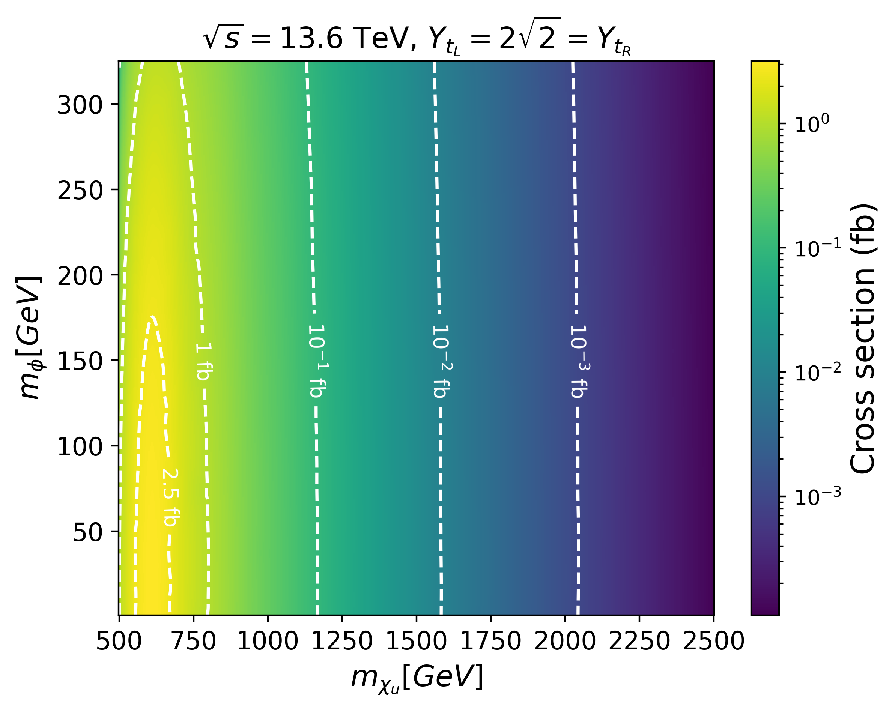
\includegraphics[width=0.85\linewidth]{Images/cross_section_by_masses.pdf}
    \caption{Projected cross section (fb) plot for $pp\to t \chi_\mathrm{u} \phi'$ and subsequent decay as a function of $m(\chi_\mathrm{u})$ and $m(\phi')$.}
    \label{fig:xs-plot}
\end{figure}

\begin{table}[]
  \begin{tabular}{l r}
    \hline
    {Background Process} & {Cross-Section $\sigma$ [\textrm{pb}]} \\
    \hline
   $\mathrm{pp} \to \mathrm{t} \overline{\mathrm{t}} \, \mu^+ \mu^-$ & $2.574\times 10^{-3}$  \\
    $\mathrm{pp} \to \mathrm{b}\overline{\mathrm{b}}\, \mu\mu\mu\nu $ & $4.692 \times 10^{-4}$ \\
    \hline
  \end{tabular}
  \centering
  \caption{A summary of dominant SM backgrounds produced by $\mathrm{pp}$ collisions and their cross sections in pb, as computed by \texttt{MadGraph} with $n = 10^6$ events.}
  \label{tab:dominantbkgs}
\end{table}

\begin{figure}[]
\centering
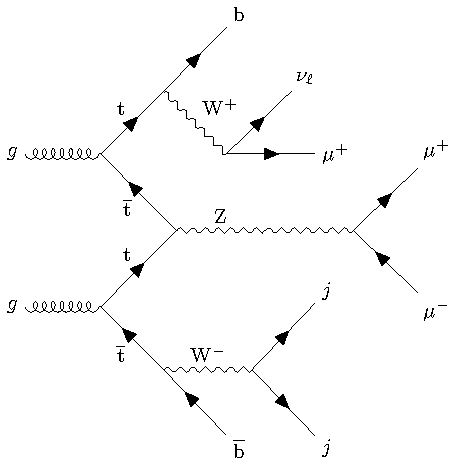
\includegraphics[width=.75\linewidth]{Images/bg_Z_full.pdf}
\caption{Representative Feynman diagram for a background event. A $Z$ boson is produced in association with a top quark through the fusion of a top, anti top pair from incoming protons. The $Z$ boson subsequently decays to a pair of muons and the two spectator top quarks decay semi-leptonically and purely hadronically to muons, neutrinos and jets, resulting in the same final states as the signal event.\label{fig:v}}
\end{figure}
